\documentclass[graphics]{beamer}
\usepackage{xcolor}
\usepackage{graphicx}
\usepackage{verbatim}
\usepackage{wrapfig}
\usepackage{tabularx}
\usepackage{multirow}
\usepackage{amssymb}
\usepackage{pifont}
\usepackage{tikz}
\def\Checkmark{\tikz\fill[scale=0.2](0,.35) -- (.25,0) -- (1,.7) -- (.25,.15) -- cycle;} 

\useoutertheme{shadow}
%\usecolortheme{orchid}
\usecolortheme{seahorse}
\newcommand{\cmark}{\text{\ding{51}}}
%\newcommand*{\GtrSim}{\smallrel\gtrsim}

% math commands
\newcommand{\be}{\begin{eqnarray}}
\newcommand{\ee}{\end{eqnarray}}
\newcommand{\beq}{\begin{equation}}
\newcommand{\eeq}{\end{equation}}
\def\simless{\mathbin{\lower 3pt\hbox
      {$\rlap{\raise 5pt\hbox{$\char'074$}}\mathchar"7218$}}}
\def\simgreat{\mathbin{\lower 3pt\hbox
      {$\rlap{\raise 5pt\hbox{$\char'076$}}\mathchar"7218$}}} %> or of order

% variables

\def\toonscale{0.45}
\def\mboxy#1{\mbox{\small #1}}

\defbeamertemplate*{title page}{customized}[1][]
{
  \usebeamerfont{title}\inserttitle\par
  \usebeamerfont{subtitle}\usebeamercolor[fg]{subtitle}\insertsubtitle\par
  \bigskip
  \usebeamerfont{author}\insertauthor\par
  \usebeamerfont{institute}\insertinstitute\par
  \usebeamerfont{date}\insertdate\par
  \usebeamercolor[fg]{titlegraphic}\inserttitlegraphic
}
\begin{comment}
\AtBeginSection[]{
  \frame{
    \frametitle{Outline}
    \tableofcontents[currentsection]
  }
}
\end{comment}


\title{\textcolor{red}{Fast Radio Burst Scintillation/scattering}}
%\subtitle{}
\author[U. Pen]{{
{ K. Masui, H-S. Lin, J. Sievers}, 
\textcolor{green}{\small Y. Li, J. Yadav, L. Connor} 
\textcolor{red}{\small U. Pen, X. Chen, J. Peterson and many more}
}
\\[8mm] 
}
\date{February 14, 2017}


\begin{document}

\frame{
\vspace{-0.5in}
\begin{center}  
%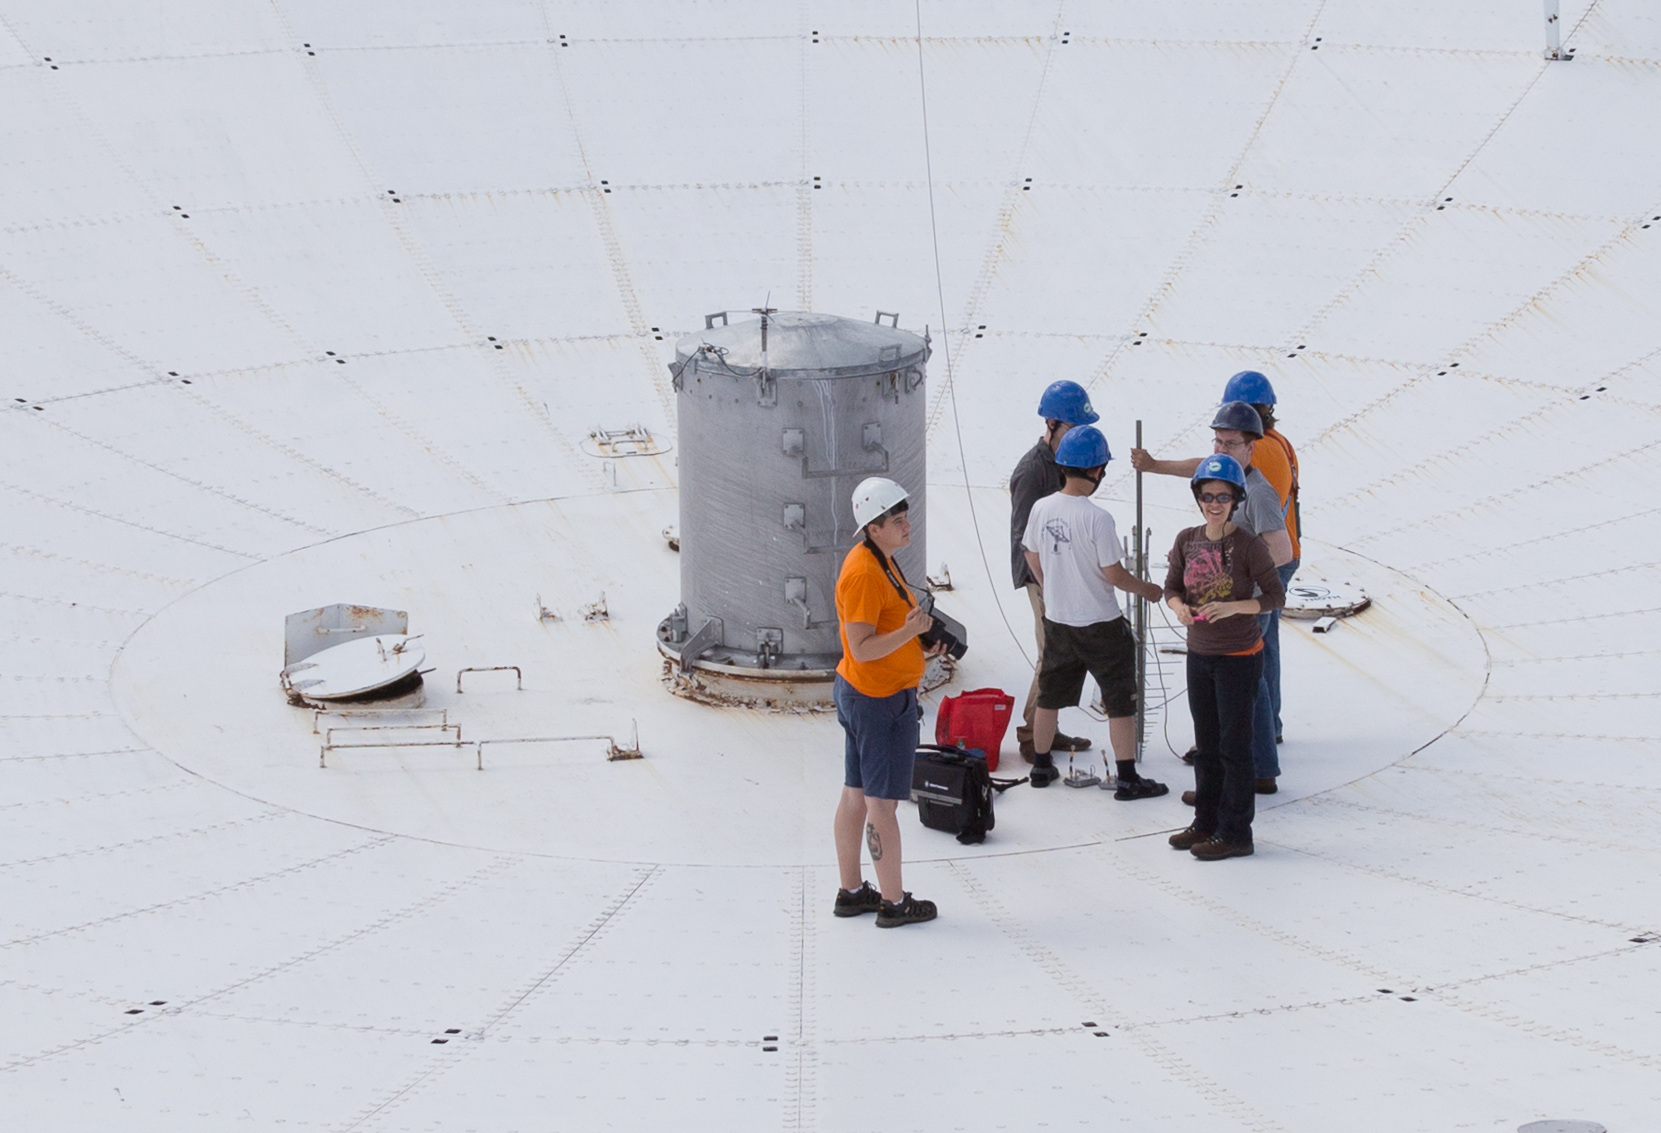
\includegraphics[width=4.4in]{Figures/IMG-0438-by-Andre-cropped.jpg}
\end{center}
\begin{picture}(320,250)
\put(-50,60){
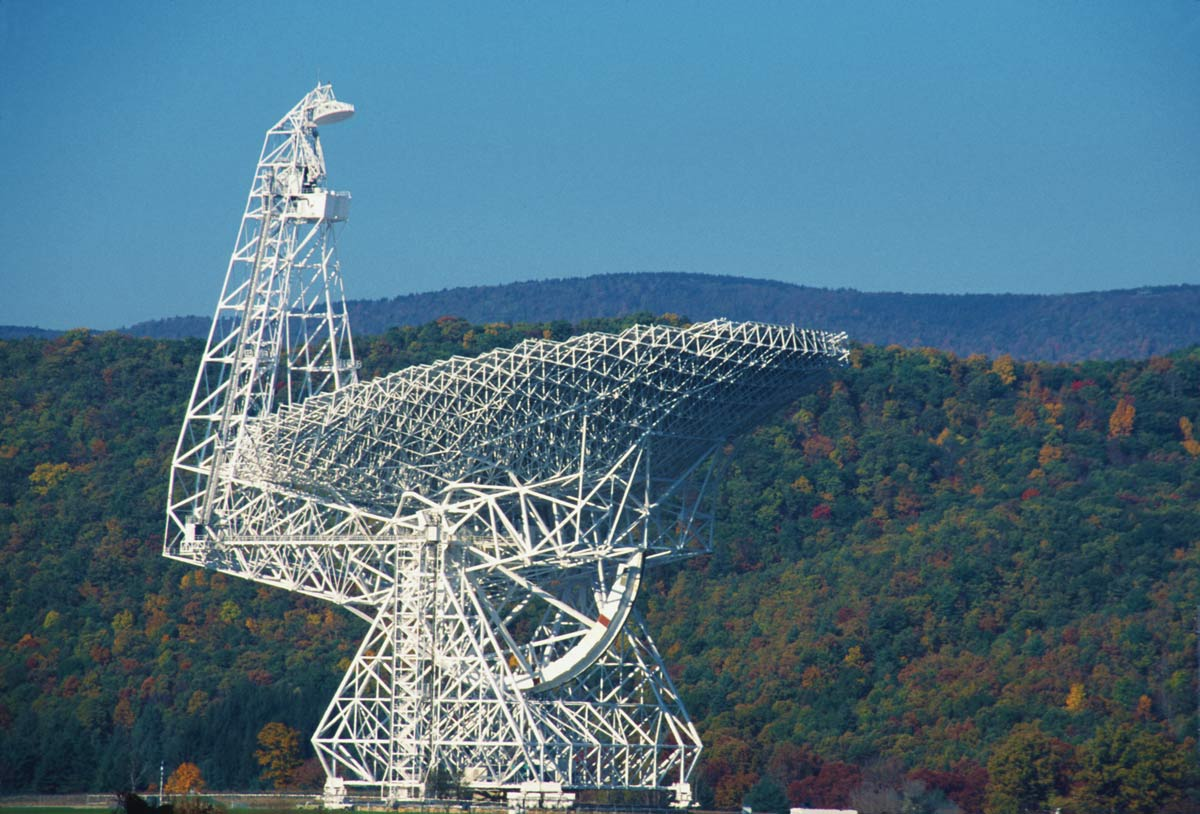
\includegraphics[width=5.5in]{Figures/GBT_nrao.jpg}}
\end{picture}
\vspace{-4in}
\\
image credit: NRAO/AUI/NSF
\\
\vspace{1in}
\titlepage
}

%\section*{Introduction}
\section{Introduction}

\begin{comment}
  \subsection{Outline}

  \frame{
    \frametitle{Outline}
    \tableofcontents
  }
\end{comment}

  \frame{
    \frametitle{Overview}
    \begin{itemize}
      \item FRB: scattering and scintillation
      \item two screen lensing
      \item FRB110523: not IGM
    \end{itemize}
  }
\section{FRBs}


\frame{
    \frametitle{FRB110523}
     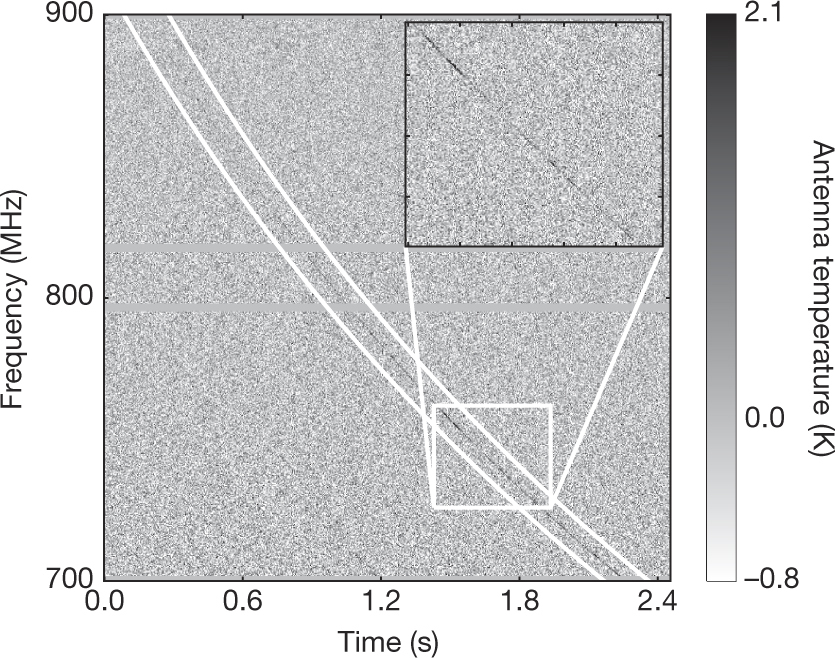
\includegraphics[width=0.8\textwidth]{Figures/nature15769-f1.jpg}

Masui et al 2015, Nature 15769
}

  \frame{
    \frametitle{FRB110523}
    \begin{itemize}
    \item Masui et al, Dec 2, 2015, Nature 15769
    \item  recorded on May 23, 2011
     \item part of GBT-IM survey, for 21cm intensity mapping (Chang et al 2010,
       Nature, 466, 463)
     \item beat double odds with data: intensity mapping, FRB       
    \end{itemize}
  }

  \frame{
    \frametitle{Two screen physics}
    \begin{itemize}
      \item long $\sim 1$ms: local to host
      \item short $\sim 1 \mu$s: galactic
    \end{itemize}
  }
\frame{
    \frametitle{Scattering}
     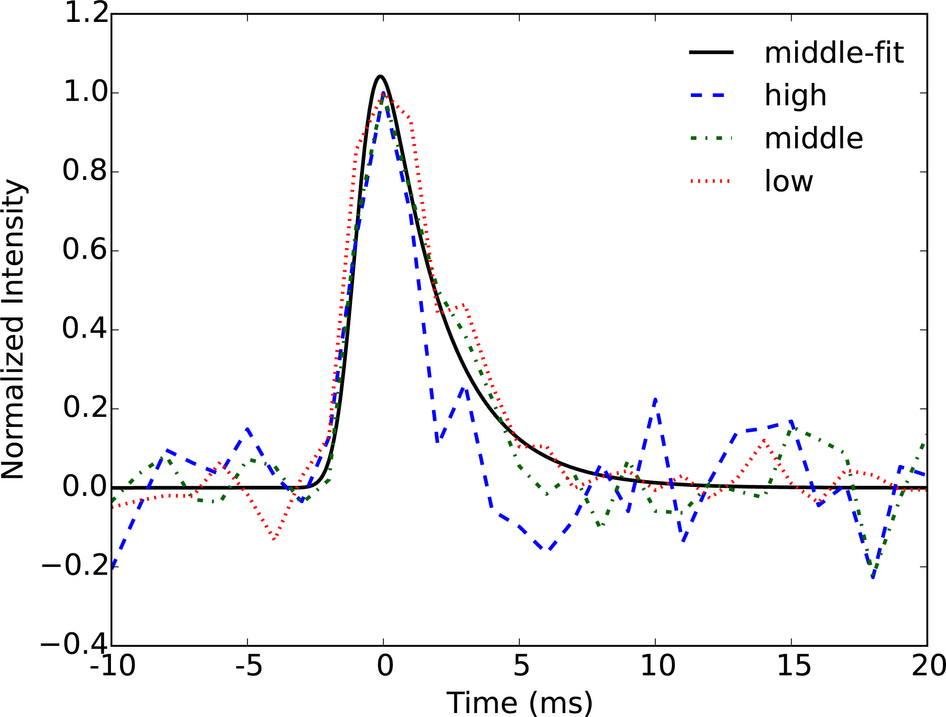
\includegraphics[width=0.8\textwidth]{Figures/nature15769-sf2.jpg}
}
  \frame{
    \frametitle{interpretation}
    \begin{itemize}
    \item ms scattering is generally due multipath propagation
    \item location was once thought to be IGM
    \item FRB110523 shows $\mu$s scintillation from Galactic multipath
    \item scattering tail scintillates!
    \item {\it stars twinkle, planets don't}
    \item constrains source size less than $\sim$ microarcsecond
    \item scattering screen is physically associated with FRB, not intergalactic
    \end{itemize}
  }
  \frame{
    \frametitle{more interpretations}
    \begin{itemize}
    \item flare stars ruled out: not enough deviation from $\lambda^2$
      law, lower bound of plasma cloud $R>10$AU, bigger than any
      plausible star
    \item scattering index consistent with refractive lensing scaling
      (Pen\&Levin 20134
    \end{itemize}
  }


\section{Summary}
  \frame{
    \frametitle{Looking forward}
    \begin{itemize}
      \item how do we reduce the allowed model space?
      \item 1. repeat rate (Connor et al 2015)
      \item 2. host galaxy
      \item 3. precision localization within host: nuclear, SNR, SFR?
      \item more unpublished bursts with new claims
      \item thousands of bursts with CHIME, HIRAX, UTMOST
      \item localization with VLBI
    \end{itemize}
  }

\frame{
    \frametitle{repeat rates}
     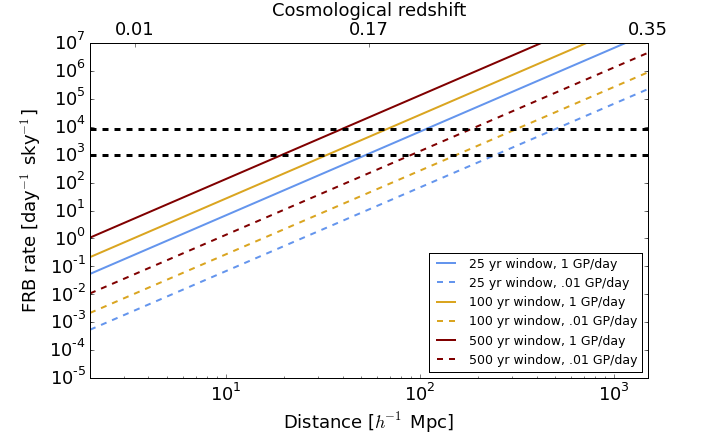
\includegraphics[width=\textwidth]{Figures/FRB_SNR_rate.png}

     Connor, Sievers, Pen 2015
}



  \frame{
    \frametitle{Conclusion}
    \begin{itemize}
      \item most plasma properties due to local environment, not
        cosmological
      \item FRBs likely extragalactic, but not cosmological        
      \item ISM structure: mapping cosmic plasma and magnetic fields
    \end{itemize}
  }

\end{document}
